% 97-49(97쪽) — 반지름의 길이가 8 인 원 위의 세 점 A·B·C 와 삼각형 ABC(원문 「오른쪽 그림」). 스캔 화질이 낮아 TikZ 로 다시 그림.
% 라벨은 원문 것만: 꼭짓점 A·B·C 와 반지름의 $8$(원문대로 점선). 세 호의 비는 원문 그림에도 적혀 있지 않다.
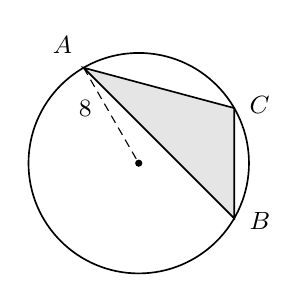
\begin{tikzpicture}[line width=0.6pt, x=1cm, y=1cm]
  \coordinate (A) at (-0.700,1.212);
  \coordinate (C) at (1.212,0.700);
  \coordinate (B) at (1.212,-0.700);
  \fill[black!10] (A) -- (C) -- (B) -- cycle;
  \draw (0,0) circle (1.4);
  \draw (A) -- (C) -- (B) -- cycle;
  \draw[densely dashed, line width=0.4pt] (A) -- (0,0);
  \fill (0,0) circle (1.3pt);
  \node[font=\small] at (-0.68,0.70) {$8$};
  \node[font=\small, anchor=south east] at (-0.72,1.26) {$\pt{A}$};
  \node[font=\small, anchor=west] at (1.28,0.74) {$\pt{C}$};
  \node[font=\small, anchor=west] at (1.28,-0.74) {$\pt{B}$};
\end{tikzpicture}
